\documentclass[11pt,a4paper]{article}

% --- Packages ---
\usepackage[utf8]{inputenc}
\usepackage[T1]{fontenc}
\usepackage{lmodern}
\usepackage[margin=2.2cm]{geometry}
\usepackage{xcolor}
\usepackage{parskip}
\usepackage{enumitem}
\usepackage{booktabs}
\usepackage{array}
\usepackage{tabularx}
\usepackage{tikz}
\usetikzlibrary{arrows.meta, positioning, shapes.geometric, calc}
\usepackage[most]{tcolorbox}
\tcbuselibrary{skins, breakable}
\usepackage[hidelinks,colorlinks=true,urlcolor=blue!60!black,linkcolor=black]{hyperref}
\usepackage{titling}
\usepackage{titlesec}

% --- Colors ---
\definecolor{accent}{HTML}{2A6F97}
\definecolor{accent2}{HTML}{61A5C2}
\definecolor{warnbg}{HTML}{FFF4E6}
\definecolor{warnframe}{HTML}{D97706}
\definecolor{tipbg}{HTML}{ECFDF5}
\definecolor{tipframe}{HTML}{059669}
\definecolor{promptbg}{HTML}{F4F4F8}
\definecolor{promptframe}{HTML}{6B7280}
\definecolor{toolbg}{HTML}{EAF3F9}

% --- Boxes ---
\newtcolorbox{watchout}[1][]{
  enhanced, breakable,
  colback=warnbg, colframe=warnframe,
  fonttitle=\bfseries, title=Watch out,
  left=8pt, right=8pt, top=4pt, bottom=4pt,
  boxrule=0.5pt, arc=2pt, #1
}
\newtcolorbox{tipbox}[1][]{
  enhanced, breakable,
  colback=tipbg, colframe=tipframe,
  fonttitle=\bfseries, title=Tip,
  left=8pt, right=8pt, top=4pt, bottom=4pt,
  boxrule=0.5pt, arc=2pt, #1
}
\newtcolorbox{promptbox}[1][]{
  enhanced, breakable,
  colback=promptbg, colframe=promptframe,
  fonttitle=\bfseries, title=Copy-paste prompt,
  left=8pt, right=8pt, top=4pt, bottom=4pt,
  boxrule=0.5pt, arc=2pt, fontupper=\small\ttfamily, #1
}
\newtcolorbox{toolheader}[1][]{
  enhanced,
  colback=toolbg, colframe=accent,
  left=10pt, right=10pt, top=6pt, bottom=6pt,
  boxrule=0.6pt, arc=3pt, #1
}

% --- Titles ---
\titleformat{\section}
  {\Large\bfseries\color{accent}}{\thesection}{0.6em}{}
\titleformat{\subsection}
  {\large\bfseries\color{accent!85!black}}{\thesubsection}{0.6em}{}

% --- Document metadata ---
\title{\textbf{From Topic to Talk in One Pipeline}\\[2pt]
\large A 45-minute practical with seven AI research tools}
\author{LOURIM --- AI for Research Seminar Series, Part 1\\\small Practical session, Corentin Vande Kerckhove}
\date{\today}

\begin{document}
\maketitle

\begin{tcolorbox}[colback=accent!8, colframe=accent!50, left=10pt, right=10pt, top=6pt, bottom=6pt, boxrule=0.4pt, arc=3pt]
\textbf{What you will do today.} You received a research topic on a slip of paper, randomly assigned by a peer. By the end of this session you will have \emph{started} a pipeline that ends, at home, with a short paper draft and a slide deck on that topic --- which you will email to a researcher working in the field. The seven tools below each take care of one step.
\end{tcolorbox}

\tableofcontents
\vspace{0.5em}

% =====================================================================
\section{Overview}
\label{sec:overview}

\subsection{The pipeline}

\begin{center}
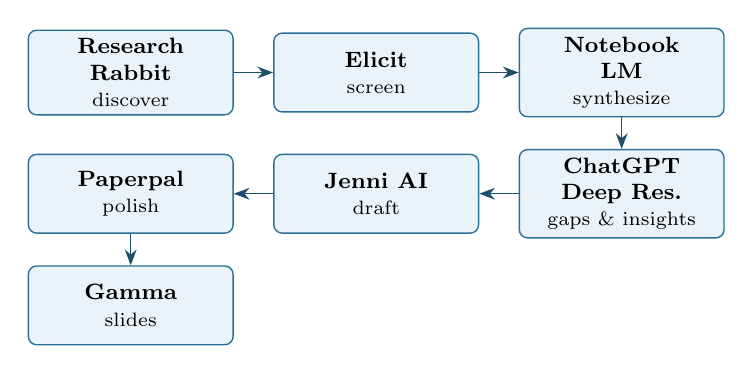
\begin{tikzpicture}[
  node distance=4mm and 5mm,
  every node/.style={font=\footnotesize},
  tool/.style={
    rectangle, rounded corners=3pt,
    draw=accent, fill=toolbg, line width=0.5pt,
    minimum width=2.6cm, minimum height=1.0cm,
    align=center, inner sep=3pt
  },
  arr/.style={-{Stealth[length=2mm]}, draw=accent!70!black, line width=0.5pt}
]
\node[tool] (rr)   {\textbf{Research}\\\textbf{Rabbit}\\\scriptsize discover};
\node[tool, right=of rr]   (el) {\textbf{Elicit}\\\scriptsize screen};
\node[tool, right=of el]   (nb) {\textbf{Notebook}\\\textbf{LM}\\\scriptsize synthesize};
\node[tool, below=of nb]   (cg) {\textbf{ChatGPT}\\\textbf{Deep Res.}\\\scriptsize gaps \& insights};
\node[tool, left=of cg]    (jn) {\textbf{Jenni AI}\\\scriptsize draft};
\node[tool, left=of jn]    (pp) {\textbf{Paperpal}\\\scriptsize polish};
\node[tool, below=of pp]   (gm) {\textbf{Gamma}\\\scriptsize slides};

\draw[arr] (rr) -- (el);
\draw[arr] (el) -- (nb);
\draw[arr] (nb) -- (cg);
\draw[arr] (cg) -- (jn);
\draw[arr] (jn) -- (pp);
\draw[arr] (pp) -- (gm);
\end{tikzpicture}
\end{center}

\subsection{Time budget}

The 45-minute session is a \textbf{kickoff}: we get the first three tools moving on your topic. The rest is guided homework you finish over the following days.

\begin{center}
\small
\begin{tabularx}{\linewidth}{@{}l X r@{}}
\toprule
\textbf{Phase} & \textbf{What happens} & \textbf{Time} \\
\midrule
Intro & Recap pipeline; check accounts; assign folder & 3 min \\
\S\,\ref{sec:rr} Research Rabbit & Seed your topic, pull \(\sim\)15 papers & 12 min \\
\S\,\ref{sec:elicit} Elicit & Two-pass screening to a 5--8 paper shortlist & 15 min \\
\S\,\ref{sec:nblm} NotebookLM (start) & Upload corpus, draft synthesis questions & 10 min \\
Homework brief & Finish NotebookLM \(\to\) ChatGPT DR \(\to\) Jenni \(\to\) Paperpal \(\to\) Gamma \(\to\) email & 5 min \\
\midrule
Homework & At your own pace, target \(\sim\)3--5\,h spread over a week & --- \\
\bottomrule
\end{tabularx}
\end{center}

\subsection{Golden rule}

\begin{tipbox}
\textbf{You are the editor; the AI drafts.} Every output of every tool is a starting point you read, prune, and correct. If you cannot defend a sentence to a colleague, delete it.
\end{tipbox}

% =====================================================================
\section{Before you start}
\label{sec:setup}

\begin{enumerate}[leftmargin=*, itemsep=2pt]
  \item \textbf{Topic in hand.} The slip of paper a peer gave you. If it is too broad (e.g.\ ``leadership''), narrow it to one question (e.g.\ ``how does remote-work intensity moderate transformational leadership effects on team performance?'').
  \item \textbf{Browser ready} with logins for the seven tools. Free tiers are enough; account links are in Appendix~\ref{app:accounts}.
  \item \textbf{One folder per participant} on your laptop or cloud drive: \texttt{my-topic/}. Subfolders: \texttt{papers/}, \texttt{exports/}, \texttt{drafts/}, \texttt{slides/}.
  \item \textbf{A prompt log.} Open a plain-text file \texttt{prompts.md} and copy every non-trivial prompt you send. This is your traceability trail.
  \item \textbf{Do not upload sensitive or unpublished data} (your own or the institute's) to any of these tools. Stick to public papers and your own notes.
\end{enumerate}

% =====================================================================
\section{Research Rabbit --- discover the literature}
\label{sec:rr}

\begin{toolheader}
\textbf{Goal.} Map the literature around your topic in 10 minutes.\\
\textbf{Input.} 1 topic phrase, or 1 known seed paper (DOI / title).\\
\textbf{Output.} A collection of \(\sim\)15 candidate papers exported to CSV / Zotero.
\end{toolheader}

\subsection*{Sign up}
Go to \href{https://www.researchrabbitapp.com/}{researchrabbitapp.com} \(\to\) ``Sign up''. Free.

\subsection*{Steps}
\begin{enumerate}[leftmargin=*, itemsep=2pt]
  \item Click \emph{Create new collection}, name it after your topic.
  \item Click \emph{Add papers} \(\to\) search by title or paste a DOI of a paper you already know is relevant. Add it.
  \item Open the seed paper in the collection. Use \emph{Similar Work}, \emph{Earlier Work}, and \emph{Later Work} to grow the network.
  \item Sort by citation count; skim titles and abstracts; add 10--15 promising ones to the collection.
  \item Open \emph{All References} or \emph{Suggested}; repeat one round.
  \item Export: collection menu \(\to\) \emph{Export to Zotero} (or CSV) \(\to\) save into \texttt{exports/research-rabbit.csv}.
\end{enumerate}

\begin{tipbox}
If you have no seed paper, search Google Scholar for ``\emph{your topic} review'' or ``\emph{your topic} meta-analysis'' and use the most cited recent review as your seed.
\end{tipbox}

\begin{watchout}
\textbf{Coverage bias.} Research Rabbit's graph is good but not exhaustive --- niche or non-English work may be missing. Cross-check one or two queries on Google Scholar or Semantic Scholar before screening.
\end{watchout}

\textit{Time budget: 12 min.}

% =====================================================================
\section{Elicit --- screen and extract}
\label{sec:elicit}

\begin{toolheader}
\textbf{Goal.} Turn 15 candidate papers into a 5--8 paper shortlist with a structured comparison table.\\
\textbf{Input.} Paper list (CSV / DOIs / PDFs).\\
\textbf{Output.} A screening table (rows = papers, columns = method / sample / findings / etc.).
\end{toolheader}

\subsection*{Sign up}
Go to \href{https://elicit.com/}{elicit.com} \(\to\) ``Sign up''. Free tier covers this exercise.

\subsection*{Steps}
\begin{enumerate}[leftmargin=*, itemsep=2pt]
  \item Create a new \emph{Workflow} (or ``List of papers'') and import your DOIs from the Research Rabbit export. Or upload the PDFs directly.
  \item Add columns. Recommended starter set:
    \begin{itemize}[leftmargin=1.4em, itemsep=1pt]
      \item \emph{Research question}
      \item \emph{Study type} (empirical / theoretical / review / meta)
      \item \emph{Method \& sample}
      \item \emph{Main finding}
      \item \emph{Limitations}
      \item \emph{Year}
    \end{itemize}
  \item Run the extraction. Skim the cells and fix obvious errors --- Elicit can over-confidently mis-summarize.
  \item \textbf{Pass 1 (title + abstract):} mark papers as \emph{keep / drop / maybe}. Drop the obvious off-topic ones.
  \item \textbf{Pass 2 (full text on \emph{keeps}):} read the method and findings cells, verify against the actual PDF for at least 3 papers, drop weak studies, end with 5--8 papers you trust.
  \item Export the table to CSV \(\to\) \texttt{exports/elicit-table.csv}. Save the kept PDFs to \texttt{papers/}.
\end{enumerate}

\begin{watchout}
\textbf{Hallucinated extractions.} Elicit's column values are model-generated summaries, not direct quotes. Always verify any number, sample size, or finding you intend to cite by opening the PDF.
\end{watchout}

\textit{Time budget: 15 min.}

% =====================================================================
\section{NotebookLM --- synthesize your corpus}
\label{sec:nblm}

\begin{toolheader}
\textbf{Goal.} Get a coherent picture of what your 5--8 papers say collectively.\\
\textbf{Input.} The shortlisted PDFs + the Elicit CSV.\\
\textbf{Output.} Saved notes covering themes, debates, consensus, and gaps.
\end{toolheader}

\subsection*{Sign up}
Go to \href{https://notebooklm.google.com/}{notebooklm.google.com}. Sign in with a Google account. Free.

\subsection*{Steps}
\begin{enumerate}[leftmargin=*, itemsep=2pt]
  \item Click \emph{New notebook}, name it after your topic.
  \item Upload all shortlisted PDFs \emph{and} the Elicit CSV as sources.
  \item In the chat panel, run the four prompts in the next box, one by one. After each, click the \emph{pin / save} icon to add the answer to your \emph{Notes}.
  \item In \emph{Notes}, manually trim and reorganize. Keep only the points that are supported by citations to your sources.
  \item Export your notes as text \(\to\) \texttt{exports/notebooklm-notes.md}.
\end{enumerate}

\begin{promptbox}
1. What are the 4--6 main themes that recur across these sources?\\[2pt]
2. Where do the sources agree, and where do they disagree? Cite the sources.\\[2pt]
3. Which definitions of the central concepts vary across the sources, and how?\\[2pt]
4. What questions do these papers leave unanswered?
\end{promptbox}

\begin{watchout}
\textbf{Source-grounding is not source-correctness.} NotebookLM cites your uploaded files, but its summary of a cited file can still be off. Click each citation chip and verify.
\end{watchout}

\textit{Time budget: 10 min in session to upload + run prompts; finish curation at home.}

% =====================================================================
\section{ChatGPT Deep Research --- find the gaps}
\label{sec:cgdr}

\begin{toolheader}
\textbf{Goal.} Step back from your corpus to identify gaps, methodological challenges, and cross-paper comparisons.\\
\textbf{Input.} Your synthesized notes from NotebookLM.\\
\textbf{Output.} An ``insights'' document feeding into your draft.
\end{toolheader}

\subsection*{Sign up}
\href{https://chatgpt.com/}{chatgpt.com}. Deep Research requires a paid plan; if you do not have one, run the equivalent prompt in regular ChatGPT or use \emph{Undermind} as a fallback.

\subsection*{Steps}
\begin{enumerate}[leftmargin=*, itemsep=2pt]
  \item Open ChatGPT \(\to\) tools menu \(\to\) \emph{Deep Research}.
  \item Paste the prompt below, replacing \texttt{<TOPIC>} and pasting your NotebookLM notes after it.
  \item Wait for the report (5--15 minutes). Read it critically.
  \item Open at least one cited source per claim you plan to keep. Discard anything you cannot verify.
  \item Save the cleaned output to \texttt{exports/insights.md}.
\end{enumerate}

\begin{promptbox}
You are a research assistant for a literature-review draft on <TOPIC>.\\
Below are my synthesized notes from a small curated corpus. Using these notes plus the broader literature, produce:\\
1. The 3--5 most consequential research gaps.\\
2. The main methodological challenges in the field.\\
3. A side-by-side comparison of the dominant theoretical perspectives.\\
4. Two or three concrete, testable directions for future work.\\
For every claim, cite at least one source with a working link. Flag uncertainty explicitly.\\[4pt]
=== NOTES ===\\
<paste NotebookLM notes here>
\end{promptbox}

\begin{watchout}
\textbf{Fabricated citations.} Even Deep Research occasionally invents references. Open each link before keeping the claim; if the link 404s or the paper does not say what is claimed, drop it.
\end{watchout}

\textit{Time budget: 15 min active + waiting time. Homework.}

% =====================================================================
\section{Jenni AI --- draft the paper}
\label{sec:jenni}

\begin{toolheader}
\textbf{Goal.} Produce a structured first draft (\(\sim\)1\,500--2\,000 words).\\
\textbf{Input.} NotebookLM notes + ChatGPT DR insights.\\
\textbf{Output.} A draft mini-paper with sections.
\end{toolheader}

\subsection*{Sign up}
\href{https://jenni.ai/}{jenni.ai}. Free tier limited to a small daily word count --- enough for one mini-paper.

\subsection*{Steps}
\begin{enumerate}[leftmargin=*, itemsep=2pt]
  \item Create a new document. Set title = your topic.
  \item Paste your NotebookLM notes and ChatGPT DR insights into the side panel as ``context'' / ``library''.
  \item Create the section headings: \emph{Introduction}, \emph{Background}, \emph{Synthesis of the Literature}, \emph{Gaps and Open Questions}, \emph{Proposed Direction}, \emph{Conclusion}.
  \item Under each heading, write one sentence stating what you want to say, then use Jenni's autocomplete to expand it. Accept, edit, or reject suggestion by suggestion.
  \item Insert citations from your shortlist as you go (Jenni links to your library or to its own search).
  \item Export to \texttt{.docx} \(\to\) \texttt{drafts/paper-v1.docx}.
\end{enumerate}

\begin{tipbox}
Write the first sentence of each paragraph yourself. It anchors Jenni and dramatically reduces hallucinated content.
\end{tipbox}

\begin{watchout}
\textbf{Citation drift.} Jenni may insert a real-looking citation that does not actually support the sentence. Re-check every citation against your shortlist.
\end{watchout}

\textit{Time budget: 60--90 min. Homework.}

% =====================================================================
\section{Paperpal --- polish the language}
\label{sec:paperpal}

\begin{toolheader}
\textbf{Goal.} Bring tone, clarity, and grammar up to academic standard.\\
\textbf{Input.} Jenni's \texttt{paper-v1.docx}.\\
\textbf{Output.} \texttt{paper-final.docx} + \texttt{paper-final.pdf}.
\end{toolheader}

\subsection*{Sign up}
\href{https://paperpal.com/}{paperpal.com}. Free tier covers one paper; the Word add-in is the smoothest path.

\subsection*{Steps}
\begin{enumerate}[leftmargin=*, itemsep=2pt]
  \item Upload \texttt{paper-v1.docx} or open it in Word with the Paperpal add-in.
  \item Run \emph{Language quality check}; accept suggestions one by one --- skip any that change meaning.
  \item Run \emph{Pre-submission} or \emph{Subject-area} check.
  \item Use \emph{Paraphrase} only on awkward sentences, not whole paragraphs.
  \item Export as \texttt{.docx} and \texttt{.pdf} into \texttt{drafts/}.
\end{enumerate}

\begin{watchout}
\textbf{Tone smoothing erodes voice.} Paperpal will gladly rewrite hedged claims into stronger ones. Re-read the diff; if a suggestion changes a ``may'' into ``does'', reject it.
\end{watchout}

\textit{Time budget: 30 min. Homework.}

% =====================================================================
\section{Gamma --- generate the slide deck}
\label{sec:gamma}

\begin{toolheader}
\textbf{Goal.} A 7--10 slide deck mirroring the paper.\\
\textbf{Input.} \texttt{paper-final.pdf} (or its text).\\
\textbf{Output.} \texttt{slides.pdf}.
\end{toolheader}

\subsection*{Sign up}
\href{https://gamma.app/}{gamma.app}. Free tier gives enough credits for one deck.

\subsection*{Steps}
\begin{enumerate}[leftmargin=*, itemsep=2pt]
  \item Click \emph{Create new} \(\to\) \emph{Generate} \(\to\) \emph{Text transform}.
  \item Paste the full text of your paper (or a 1-page summary).
  \item Set: number of cards = 8--10, tone = \emph{academic}, audience = \emph{researchers}.
  \item Generate. Open the deck.
  \item Edit the title slide (your name, topic, date, LOURIM). Add or remove cards so the deck mirrors the paper sections.
  \item Replace any AI-chosen image you cannot defend. When in doubt, no image.
  \item Export \(\to\) \texttt{slides/slides.pdf}.
\end{enumerate}

\begin{tipbox}
You can run Gamma in parallel with Paperpal: launch the Gamma generation, switch to Paperpal while Gamma works.
\end{tipbox}

\begin{watchout}
\textbf{Generated visuals can mislead.} Charts and diagrams produced from prose are decorative, not analytical. Do not present a generated chart as if it were data.
\end{watchout}

\textit{Time budget: 30 min. Homework.}

% =====================================================================
\section{Send to the researcher}
\label{sec:send}

The final deliverable is an email, sent within roughly one week of the session, to a researcher working on your topic.

\subsection*{Identify the recipient}
Pick the researcher you (or the organizer) identified for your topic --- most often the most-cited author from your shortlist whose institutional email is reachable. One person is enough.

\subsection*{Attachments checklist}
\begin{itemize}[leftmargin=*, itemsep=1pt]
  \item \texttt{paper-final.pdf}
  \item \texttt{slides.pdf}
\end{itemize}

\subsection*{Email template}

\begin{promptbox}
Subject: Student exploration on <TOPIC> --- LOURIM AI seminar (your feedback?)\\[4pt]
Dear Prof. <NAME>,\\[2pt]
As part of an AI-for-research seminar at LOURIM (UCLouvain), I produced a short literature synthesis on <TOPIC>, drawing notably on your work on <SPECIFIC PAPER>.\\[2pt]
The paper draft and a short slide deck are attached. The exercise was time-boxed and AI-assisted, so it is exploratory rather than a finished review --- I would value any feedback you might have on the framing, gaps, or proposed direction.\\[2pt]
With thanks for your time,\\
<YOUR NAME>\\
LOURIM, UCLouvain
\end{promptbox}

\begin{watchout}
\textbf{Disclose AI use.} The email already says ``AI-assisted''; keep that line. Researchers appreciate transparency far more than they mind the use of tools.
\end{watchout}

% =====================================================================
\section{Risks: a six-line reminder}
\label{sec:risks}

\begin{center}
\small
\begin{tabularx}{\linewidth}{@{}l X@{}}
\toprule
\textbf{Hallucinations} & Verify every fact, number, and citation against the original source. \\
\textbf{Bias} & Models reflect their training corpus --- be explicit about whose voices may be missing. \\
\textbf{Confidentiality} & Never upload unpublished data, sensitive interviews, or institute documents. \\
\textbf{Traceability} & Keep \texttt{prompts.md} updated; future you will need it. \\
\textbf{Scientific integrity} & The argument and the literature claims are yours to defend. \\
\textbf{Responsibility} & Your name is on the paper. The tool's is not. \\
\bottomrule
\end{tabularx}
\end{center}

% =====================================================================
\appendix

\section{Accounts and free tiers}
\label{app:accounts}

\begin{center}
\small
\begin{tabularx}{\linewidth}{@{}l l X@{}}
\toprule
\textbf{Tool} & \textbf{Sign-up} & \textbf{Free-tier note} \\
\midrule
Research Rabbit   & researchrabbitapp.com  & Fully free. \\
Elicit            & elicit.com             & Free monthly credits, enough for one screening. \\
NotebookLM        & notebooklm.google.com  & Free with a Google account. \\
ChatGPT Deep Res. & chatgpt.com            & Paid plan; fallback: regular ChatGPT or Undermind. \\
Jenni AI          & jenni.ai               & Free daily word cap; fits one mini-paper. \\
Paperpal          & paperpal.com           & Free checks per month + Word add-in. \\
Gamma             & gamma.app              & Free credits cover one deck. \\
\bottomrule
\end{tabularx}
\end{center}

\section{Troubleshooting}
\label{app:troubleshoot}

\begin{itemize}[leftmargin=*, itemsep=2pt]
  \item \textbf{Research Rabbit shows few similar papers.} Add a second seed paper; the network grows multiplicatively.
  \item \textbf{Elicit credits exhausted.} Run extraction on the 5--8 most relevant papers only, not all 15.
  \item \textbf{NotebookLM upload failure.} Split a large PDF, or convert a scanned PDF to text first (e.g.\ Adobe / a free OCR tool).
  \item \textbf{Deep Research unavailable.} Use \emph{Undermind} (\href{https://undermind.ai/}{undermind.ai}) or run the same prompt in standard ChatGPT with \emph{Browse} on.
  \item \textbf{Jenni inserts unknown citations.} Disable autocomplete's web citation source; keep only your library.
  \item \textbf{Paperpal changes meaning.} Reject the suggestion; rewrite by hand. Never accept the entire diff at once.
  \item \textbf{Gamma export looks bad.} Use \emph{Export to PDF}, not \emph{Print} from the browser.
\end{itemize}

\vspace{1em}
\hrule
\vspace{0.5em}
\small \textit{LOURIM --- AI for Research Seminar Series, Part 1.} Source: \href{https://github.com/cvandekerckh/lourim-ai-seminar-series}{github.com/cvandekerckh/lourim-ai-seminar-series}.

\end{document}
